\documentclass[11pt,a4paper]{article}
\usepackage[T1]{fontenc}
\usepackage[utf8]{inputenc}
\usepackage{lmodern}
\usepackage{microtype}
\usepackage[margin=2.6cm]{geometry}
\usepackage{amsmath}
\usepackage{booktabs}
\usepackage{tabularx}
\usepackage{array}
\usepackage{enumitem}
\usepackage{graphicx}
\usepackage{xcolor}
\usepackage{textcomp}
\usepackage{listings}
\usepackage{tikz}
\usepackage{pgfplots}
\usepackage{pgfplotstable}
\pgfplotsset{compat=1.17}
\usetikzlibrary{arrows.meta,positioning}
\usepackage[numbers,sort&compress]{natbib}
\usepackage{xurl}
\usepackage[hidelinks]{hyperref}
\usepackage{caption}
\captionsetup{font=small,labelfont=bf}
\lstset{basicstyle=\ttfamily\footnotesize,breaklines=true,columns=fullflexible,frame=single,framesep=3pt,rulecolor=\color{black!25},xleftmargin=4pt,xrightmargin=4pt,extendedchars=true,upquote=true,literate={ã}{{\~a}}1 {ç}{{\c{c}}}1 {é}{{\'e}}1}
\setlength{\emergencystretch}{2em}

\title{\textbf{Check It Yourself:\\ Verifiable Legislative Transparency\\ in Simple Language for Brazil's Chamber of Deputies}}
\author{Rafael Coutinho\\[2pt]
{\small Independent researcher, Brazil}\\
{\small\texttt{rafaelcouto111@gmail.com}}}
\date{November 2026}

\begin{document}
\maketitle

\begin{abstract}
\noindent
Most Brazilians cannot name a single member of the Chamber of Deputies, and the intermediaries that could bring the legislature closer are distrusted. We present \emph{Vigia do Povo}, an open-source site that tells citizens, in simple language, what the Chamber votes and how each deputy voted, and whose daily data files readers can check without trusting its operator. The collector runs on a machine hosted by the CI platform; each daily collection is content-addressed with SHA-256, attested through Sigstore to the public code and run that produced it, and timestamped in Bitcoin with OpenTimestamps. Metrics since 2003 are public formulas that anyone can recompute from the Chamber's files. The guarantees are not uniform: the historical metrics are checkable by recomputation, not by signature; the pages are deployed by the operator and are not attested; and, because the Chamber does not sign its data, no proof reaches back to what the Chamber said. We prove the commitment properties in Lean. Using only public data, we verified the current collection's attestations, its 254 file digests and twelve timestamps, and recomputed 363 published rows of the metric from 336,089 official vote records, finding no difference. We argue that the realistic value of verifiability lies with journalists, fact-checkers and other intermediaries.
\end{abstract}

\noindent\textbf{Keywords:} legislative transparency; data provenance; Sigstore; trusted timestamping; formal verification; civic technology; disinformation; Brazil.

\section{Introduction}
\label{sec:intro}

In June 2026, four months before a general election, two in three Brazilian voters could not remember whom they had chosen for the Chamber of Deputies four years earlier, and two in three could not name a single sitting deputy~\citep{folha2026votememory}. That October a presidential election was decided by fewer than four points, and the defeated candidate alleged fraud without presenting evidence~\citep{tse2026runoff,cnn2026letter}; four years earlier, an even closer result had been followed by an attack on the seats of all three branches of government~\citep{tse2022result,stf8jan}. Trust in news stood at a twelve-year low~\citep{carro2026brazil}, and fact-checkers were counting about twenty AI-made political items a day~\citep{lupa2026vigia}.

These facts describe one problem from two sides. Citizens are far from the institution that writes their laws, and the channels that could bring them closer are not believed. The records exist: the Chamber publishes every recorded vote as open data. But raw records are not understanding, and whoever turns one into the other, a newspaper, a ranking or a message forwarded in a family group, asks to be trusted at a moment when trust is the scarce resource.

\emph{Vigia do Povo} (``the people's watch'') is an independent, open-source site built to address both sides. Its first aim is to shorten the distance: to tell a citizen, in simple language and with the context needed to read it, what the Chamber voted and how each deputy voted. Its second aim is that the reader should not have to trust the site to believe the data behind it. The daily collection's data files and the published metrics come with the means to check them:

\begin{itemize}[leftmargin=1.4em,itemsep=2pt]
\item every collected file is named by its SHA-256 digest, and one manifest digest commits to a whole day's collection;
\item the collector is open source and runs on a machine hosted by GitHub, not by the maintainer; a signed attestation, recorded in a public transparency log, binds each collection to the source code, commit and automated run that produced it, so that a file edited by hand is detectable;
\item a timestamp anchored in the Bitcoin blockchain shows that the collection existed by a given time, and remains checkable if the project and every service it uses disappear;
\item an append-only store keeps every version of the official yearly files it has seen, so that later changes to the official record are visible;
\item every metric is a public formula over the official files, which a reader can recompute with unrelated tools.
\end{itemize}

The guarantees are not uniform, and we keep them apart throughout. The daily collection carries the full chain of signed provenance and timestamp. The historical metrics since 2003 are computed from the Chamber's yearly files and are checkable by recomputation, not by signature. The pages a reader sees are built and deployed by the operator and are not attested, and nothing shows that the collection they present is the latest. And because the Chamber does not sign what it publishes, no proof reaches back to what the Chamber itself said.

None of these techniques is new. They come from software supply-chain security, trusted timestamping and data engineering. What we contribute is their combination for a setting that we believe is common and underserved: an outsider with no authority republishing a government's unsigned open data for a public that has reason to be sceptical. Specifically, we contribute:

\begin{enumerate}[leftmargin=1.6em,itemsep=2pt]
\item \textbf{a design} for verifiable republication of legislative data that runs entirely on free public infrastructure, with no ledger, token or signing key of its own, together with the reasons for not using an on-chain verifier;
\item \textbf{a trust analysis} that separates what is proven from what is not, including freshness, hidden inputs and long-term preservation;
\item \textbf{machine-checked proofs} in Lean of the properties the design relies on: that the manifest commits to its artifacts unless SHA-256 has a collision, that a proposed hash chain over the lake's batches would commit to them unless SHA-256 has a collision or a preimage of a fixed starting value, that a timestamp path cannot be moved to another document, and that the published metric is well defined;
\item \textbf{an evaluation of the deployed system}, in which the attestations of the current collection, all 254 of its file digests and twelve timestamps verified, a tampered file was rejected, and an independent recomputation of 363 published rows of the metric from 336,089 official vote records found no difference;
\item \textbf{an assessment of social impact} grounded in the experimental literature, which finds that information alone rarely changes votes, and an account of the risks the system itself creates.
\end{enumerate}

We first describe the Brazilian setting and the work this builds on. We then define the trust gap and present the design and the software, analyse its security, and evaluate the deployed system. We close with its expected social impact, its limitations, and a planned extension to the messaging channels where most Brazilians meet political information.

\section{The problem: a distant legislature and a contested record}
\label{sec:context}

This section describes the setting the system was built for. Every figure is taken from the source cited beside it; all web sources were read on 16 November 2026.

\subsection{The distance between citizens and their deputies}

In June 2026, 67\% of Brazilian voters did not remember whom they had voted for federal deputy four years earlier, and 68\% could not name a single sitting deputy. Only 7\% had forgotten their vote for president. Six of the 513 deputies were named by at least 1\% of respondents~\citep{folha2026votememory}. The pattern is old: in the 2014 national election study, more than 40\% could not recall their vote for deputy a few weeks after casting it~\citep{fapesp2015eseb}.

Distance comes with distrust. In September 2026, 45\% of voters said they do not trust the National Congress and 45\% that they do not trust political parties~\citep{datafolha2026trust}; on a 0--100 index of social trust the Congress scored 34 and the parties 30, the two worst results of the survey~\citep{ipsos2026ics}. Support for democracy in Brazil stood at 41\%, the second lowest among the Latin American countries surveyed~\citep{latinobarometro2026}, and 37\% of adults were satisfied with how democracy works~\citep{pew2026brazil}. A quarter of voters declared no interest in politics at all~\citep{datafolha2026interest}.

Part of the distance is institutional. The Chamber has 513 members elected by open-list proportional representation in state-wide districts~\citep{tse2026systems}, a system that, in one influential account, produces weak parties and individualistic politicians with little accountability to citizens~\citep{ames2001deadlock}, and in which few voters can follow the path from their vote to a seat~\citep{nicolau2017representantes}. Twenty parties won seats in 2026, down from thirty in 2018~\citep{folha2026fragmentation}; the effective number of parties fell from 16.7 to 8.8 over the same period~\citep{tejadas2026nep}, from a level that had made the Chamber the most fragmented lower house in the world~\citep{poder3602023fragmentation}. Presidents govern through broad, shifting coalitions~\citep{abranches1988presidencialismo}, so the question of who supports the government has a different answer in each legislature. The largest party in the Chamber elected in 2026 holds 121 seats, under a quarter of the house~\citep{cnn2026seats}.

Part of it is volume. Between 1988 and 2017, 56,804 ordinary bills were filed in the Chamber, of which 4.63\% were approved~\citep{cerdeira2018congresso}. Much of what is enacted is symbolic: of the 164 ordinary laws of 2010, 43 were tributes or commemorative dates~\citep{queiroz2010producao}. A citizen who counts bills filed measures activity, not results.

Part of it is opacity that the courts themselves have had to correct. Parliamentary amendments to the federal budget amount to about R\$\,61 billion in 2026~\citep{senado2026budget}. In December 2022 the Supreme Court struck down one category of them, the so-called secret budget, because the amendments were anonymous and so violated the constitutional principle of publicity~\citep{stf2022secretbudget}.

And part of it is language. In the most recent national survey, 29\% of Brazilians aged 15 to 64 were functionally illiterate and only 10\% were proficient readers~\citep{inaf2024}. A federal law of November 2025 created a national policy of \emph{simple language} (\emph{linguagem simples}) and requires every public body, in all branches and levels of government, to use it with citizens. The law defines simple language as the set of techniques for conveying information clearly and objectively, so that the words, structure and layout of a message let citizens easily find the information, understand it and use it~\citep{brasil2025lei15263}. We use the term in that sense throughout: not a register or a style, but the removal of abstractions that stand between a citizen and the information. Legislative records, written in procedural terms for specialists, are far from that standard. In the vocabulary of \citet{michener2013identifying}, they are \emph{visible} but not \emph{inferable}: the public can see them and still cannot draw accurate conclusions from them.

\subsection{Contested elections and the disinformation that surrounds them}

The distance would matter less if citizens trusted those who report on the legislature. Brazil's last two presidential elections show why they often do not.

In 2022, Luiz In\'acio Lula da Silva defeated the incumbent, Jair Bolsonaro, with 50.90\% of the valid votes, the narrowest margin since direct presidential elections resumed in 1989~\citep{tse2022result,g12022margin}. In a panel study around that election, about half of respondents rated as accurate the false statements that votes are counted in a secret room and that the voting machines cannot be audited~\citep{montalverne2024nexus}. A week after the inauguration, on 8 January 2023, rioters invaded the seats of the three branches of government~\citep{stf8jan}. Bolsonaro was later declared ineligible for attacking the voting system before foreign ambassadors~\citep{tse2023ineligible} and, in September 2025, sentenced to 27 years and three months in prison for crimes that include an attempted coup~\citep{stf2025conviction}. In October 2026 Lula won again, with 51.79\% against Fl\'avio Bolsonaro~\citep{tse2026runoff}, who had led the first round~\citep{g12026rounds}; the defeated candidate refused to concede and alleged fraud without presenting evidence~\citep{reuters2026concede,cnn2026letter}, while international observers reported no doubts about the integrity of the results~\citep{oas2026brazil}. We take no position on any candidate. What matters here is that, twice in four years, close to half the electorate saw leaders it supports cast doubt on an official record, and had no practical way to check it.

Disinformation filled that space through the channels people actually use. In 2018, images that fact-checkers had confirmed as false were fewer than 1\% of the images shared in monitored WhatsApp political groups but reached 44\% of the groups~\citep{resende2019whatsapp}, and companies were reported to be paying for bulk messaging against one party~\citep{camposmello2018empresarios}. In 2022, having joined a political WhatsApp group was the strongest predictor of believing electoral falsehoods~\citep{rossini2023electoral}, and public groups were used to organise the attack of 8 January~\citep{ozawa2024capitol}. In 2026 the content became synthetic: one fact-checking project confirmed 1,423 political items made with generative AI in the campaign, about 21 a day, of which 768 carried no label~\citep{lupa2026vigia}, despite the electoral court's rules on synthetic content~\citep{tse2024res23732,tse2026res23755}. The bill that would regulate platforms has waited for a floor vote since 2023~\citep{brasil2020pl2630}.

Corrections struggle against this. Fact-checks do reduce false beliefs on average~\citep{walter2020factchecking,porter2021global}, but falsehood spreads faster than truth~\citep{vosoughi2018spread}, 40.7\% of the shares of debunked images in Brazilian WhatsApp groups happened after the debunking~\citep{reis2020debunked}, and an experiment during the 2018 Brazilian election found corrections ``ineffective at reducing misinformation''~\citep{batistapereira2022fake}. Underneath is a problem of trust: in 2026 trust in news in Brazil fell to 36\%, a twelve-year low, while 53\% of internet users got news from social media each week and 46\% from WhatsApp~\citep{carro2026brazil}. A correction asks its reader to believe the corrector, and that request often fails before the evidence is seen.

\subsection{The gap}

The Chamber is not secretive. It publishes its records as structured open data, and Brazil's access-to-information law makes publicity the rule and secrecy the exception~\citep{brasil2011lai}. The gap is between raw publication and public understanding, and it is filled by intermediaries: newspapers, rankings, influencers and message groups. Each has a point of view, or is assumed to have one, and none can be checked by its audience.

\citet{oneill2002question} argued two decades ago that transparency alone does not build trust, and that trust has a basis only when people are offered not ``a flood of uncheckable information, but rather information whose accuracy they can check and assess for themselves''. The system described next is an attempt to build an intermediary of that second kind: one that brings the legislature closer in simple language, and that does not ask to be believed.

\section{Related work}
\label{sec:related}

\subsection{Parliamentary monitoring}

Organisations that republish and interpret parliamentary records are an established part of civil society. A 2011 survey counted more than 191 of them, monitoring over 80 national parliaments, with Latin America the most active region~\citep{mandelbaum2011strengthening}. The best known republish debates and votes in searchable form: TheyWorkForYou in the United Kingdom~\citep{mysociety_twfy}, GovTrack in the United States~\citep{govtrack_about}, OpenParliament in Canada~\citep{openparliament_about} and abgeordnetenwatch in Germany~\citep{abgeordnetenwatch_about}. Voteview publishes every roll call of the US Congress with estimated ideal points~\citep{voteview_about}.

Brazil has a rich tradition of its own. Opera\c{c}\~ao Serenata de Amor uses open data to flag suspicious expense reimbursements of legislators~\citep{serenata2016,coutinho2021public}. Radar Parlamentar maps parties by a principal-component analysis of roll calls~\citep{leite2016analise}. The newspaper tool Bas\^ometro measures how often each deputy votes with the government's orientation, with data back to 2003~\citep{estadao_basometro}, and is the closest precedent for the alignment metric we publish. Ranking dos Pol\'iticos~\citep{rankingpoliticos2026criterios} and the \'Indice Legisla Brasil~\citep{legislabrasil2025relatorio} score legislators. Parlametria aggregated legislative data for advocacy organisations from 2019 to 2023~\citep{okbr_parlametria}. Radar do Congresso offers search and analysis of legislators' records~\citep{congressoemfoco_radar}, and Querido Di\'ario republishes municipal official gazettes in open form~\citep{okbr_queridodiario}.

Two observations about this field motivate our work. First, on the public pages we could read of the projects named above (Parlametria's are offline), none describes a way for a reader to verify the published data independently: no digests, signatures, timestamps or transparency logs. The reader is asked to trust the project, its code where it is open, and its hosting. Second, monitoring projects end. VoteWatch Europe stopped in 2022 and its site now carries only a closure notice~\citep{votewatch_closure}; Parlametria's sites are offline; even the domain that hosted the international Declaration on Parliamentary Openness~\citep{openingparliament2012declaration} now serves unrelated content. When such a project disappears, so does the public's ability to check what it once published. Proofs that outlive the project address exactly this.

\subsection{Scores and rankings of legislators}

Rankings are the most popular and the most criticised product of monitoring organisations. Ranking dos Pol\'iticos assigns 75\% of a legislator's score to votes, where a council of the organisation decides which way each vote should count~\citep{rankingpoliticos2026criterios}; critics argue that such criteria embed their authors' world view while presenting themselves as neutral~\citep{queiroz2022rankings,filho2018engodo}. The \'Indice Legisla Brasil combines 17 indicators and in its 2024 edition compresses extreme values so that filing very many bills does not inflate a score~\citep{legislabrasil2025relatorio}.

The experience of TheyWorkForYou is the cautionary tale. Members of Parliament ``increased the number of times they spoke just to increase their scores''~\citep{korthagen2020parliamentary}; the site removed its explicit rankings in 2006 and all comparative statistics in 2020, concluding that ``if we do not believe data can help make meaningful evaluations or requires large qualifications, we should not highlight it''~\citep{parsons2020publishing}. This is Campbell's law~\citep{campbell1979assessing}: an indicator used for social decisions comes under pressure that corrupts both the indicator and the process it measures.

The project's own unpublished score does not escape this critique, although it is a deterministic function of official outcomes with no discretionary input and reports how each rank moves under alternative weights.

\subsection{Roll-call analysis in Brazil}

Political science has studied Brazilian roll calls for three decades. \citet{figueiredo1999executivo} used them to show that parties in the Chamber are disciplined and that the executive controls the agenda, against the view that open-list rules produce only individualists~\citep{ames2001deadlock,mainwaring1999rethinking}. \citet{zucco2011distinguishing} show that voting in the Chamber is structured less by left--right ideology than by a government--opposition dimension, on which parties jump when they enter or leave the coalition. This is the scholarly basis for publishing coincidence with the Government's orientation as the first metric, and the evaluation shows the jumps directly. Our metric is far simpler than ideal-point models~\citep{poole1997congress,clinton2004statistical} or survey-based placements~\citep{power2009estimating}. The simplicity is intended: a ratio of two counts can be recomputed by a reader with a spreadsheet, which a Bayesian item-response model cannot.

\subsection{Cryptographic provenance and verifiable records}

The components we use are well established. Tamper-evident logs~\citep{crosby2009tamper} became public infrastructure with Certificate Transparency~\citep{rfc6962,laurie2014ct}. Sigstore applies the same idea to software signing with short-lived, identity-bound certificates~\citep{newman2022sigstore}; in-toto and SLSA define what a build should attest~\citep{torresarias2019intoto,slsa12}; and The Update Framework showed how to survive key compromise in software distribution~\citep{samuel2010tuf}. Trusted timestamping predates blockchains~\citep{haber1991timestamp,rfc3161}, and Bitcoin has been used to timestamp documents since at least 2015~\citep{gipp2015timestamping}.

These tools were built for software supply chains. Their use for \emph{data} is recent: Sigstore-based model signing covers machine-learning artifacts and datasets by manifest~\citep{openssf-oms}, the SCITT architecture generalises transparency logs to arbitrary signed statements~\citep{rfc9943}, and C2PA attaches signed provenance to media~\citep{c2pa25}. All of them assume that the party vouching for the content is its producer.

The closest practices on the archiving side do not involve the producer either. ``Git scraping'' runs a scheduled CI job that fetches a source and commits the result, so that the repository's history records every change~\citep{willison2020git}; our collector is an instance of it, with attestation and timestamping added. Software Heritage archives public source code and its history under intrinsic, hash-based identifiers~\citep{dicosmo2017software}. Web archives in the WACZ format can carry a signature over the capture~\citep{wacz-signing}, which binds an archive to the party that made it but, like our attestations, cannot show what the original server sent.

Closer to our subject, several systems protect public records. ARCHANGEL uses a distributed ledger run by archives to guarantee the long-term integrity of documents in their custody~\citep{collomosse2018archangel}. Estonia protects government registries with a keyless signature infrastructure based on hash trees~\citep{buldas2013ksi,eestonia-ksi}. \citet{beris2018modeling} prototype the anchoring of Greek government decisions in Bitcoin with a verifier for citizens, and \citet{arruzzoli2026multichain} propose a multi-chain architecture for Italian legislative documents. In each case the custodian of the records, or a system acting for it, applies the protection. A critical survey of blockchain projects in government finds many benefits claimed and few demonstrated~\citep{olnes2017blockchain}.

Our situation is different, and we believe more common: the custodian publishes open data without signatures, and an outsider with no authority republishes it. We found no prior system that combines content-addressed captures, CI-identity attestations in a public transparency log, blockchain timestamps and replayable metrics for public legislative data. Our search covered the websites of the monitoring projects above and literature searches for combinations of transparency logs, Sigstore or blockchain timestamps with legislative, parliamentary or government open data; finding no counter-example is weaker than showing that none exists. We also use no ledger of our own, no token and no smart contract: only hashing, a public signing service and a timestamp.

The closest conceptual relative is end-to-end verifiable voting~\citep{benaloh2015e2e}, whose principle is that anyone can check an election outcome without trusting the software or the officials. Researchers who tested Brazil's voting machines have reported software vulnerabilities in them~\citep{aranha2019return}, and the election disputes described above turned on whether citizens could check the count. Roll-call data are an easier case, since votes on the floor are public and privacy does not constrain the design. The hard part moves elsewhere, to the authenticity of the source.

\section{Goals and threat model}
\label{sec:goals}

\subsection{The main goal: closing the distance}

The problem described above is first a problem of distance. The Chamber publishes a REST API and yearly bulk files with every voting, every individual vote and every leadership orientation~\citep{camara_dadosabertos}. The data are public, but they are large (the 96 yearly files used for the metrics add up to 1.52\,GB of JSON), spread over many endpoints, and written in procedural vocabulary. A citizen who wants to know what was voted yesterday, or how a party has voted since the last election, cannot get the answer from them unaided.

The main goal of the system is therefore to bring the legislature closer to the people it represents: to say, in simple language, what each voting was about, who voted and how, and to give the context needed to read a vote correctly, such as what the official summary of the bill says, what the leaderships oriented, and how a party has behaved over time. Verifiability serves that goal; it is not a goal in itself. An intermediary that explains the Chamber but cannot be believed does not close the distance, and in Brazil today every intermediary is presumed to have a side.

Vigia do Povo is such an intermediary, run by a private individual with no institutional standing. Its design starts from the assumption that readers have no reason to trust it, and that some will suspect it of taking a side.

\subsection{Goals}

\begin{description}[leftmargin=1.2em,style=nextline,itemsep=2pt]
\item[G1. Closeness.] A citizen with no training can find out what the Chamber voted and how each deputy voted, in simple language, with the context needed to interpret it.
\item[G2. Reach.] The site works on a cheap phone and a slow connection and never requires JavaScript to read a page.
\item[G3. Integrity.] Anyone can detect whether a published file was changed after it was collected.
\item[G4. Provenance.] Anyone can check which program, at which source revision and in which run, produced a published file, and that no person edited the output by hand.
\item[G5. Time.] Anyone can check that a collection existed no later than a given moment, without trusting the project's clock or its hosting providers.
\item[G6. History.] When the official source changes or removes a record, the earlier version stays available, and the change is itself recorded.
\item[G7. Recomputation.] Every published number follows from the official files by a public rule that a reader can apply with tools unrelated to the project.
\item[G8. Zero cost.] The system runs inside free allowances, so that it does not depend on a funder and can be replicated by anyone.
\end{description}

G1 and G2 are the purpose. G3 to G7 make the purpose credible. G8 keeps it alive: a transparency tool that stops when a grant ends does not serve the people it is for.

\subsection{Adversaries and trust}

We consider four adversaries.

\emph{The operator.} The maintainer, or someone who takes over the maintainer's accounts, may want to alter a vote, a count or a date. This is the adversary a sceptical reader has in mind, and the main one the design addresses.

\emph{The host.} The site is served by a CDN and the metrics by an object store. Either could serve altered files, by fault or under pressure.

\emph{The network.} An attacker between the reader and the site may alter responses.

\emph{The source.} The Chamber may correct, rewrite or remove records after publication. Most such changes are legitimate corrections, but a reader should be able to see them.

The design does \emph{not} defend against a source that publishes false records from the start, nor against a compromise of the continuous-integration (CI) platform that runs the collector.

\subsection{The trust gap}
\label{sec:gap}

It helps to state precisely what a reader of a conventional monitoring site takes on faith. Between the legislature's server and the reader's screen there is a chain of steps that only the operator sees:

\begin{enumerate}[leftmargin=1.6em,itemsep=1pt]
\item \emph{Which program} fetched the data, and whether it is the program the operator says it is.
\item \emph{Whether that program ran unmodified}, on the day in question, or whether something else produced the output.
\item \emph{Whether a person touched the output} between the program and the database.
\item \emph{Whether the database was changed later}, after the reader, a journalist or a court relied on it.
\item \emph{Whether the published number} was computed from that database by the rule the site describes.
\end{enumerate}

We call the sum of these the \emph{trust gap}. It exists even when the operator is honest and the code is open, because publishing source code shows what \emph{could} have run, not what \emph{did} run. An operator who publishes a scraper on a code-hosting site and runs it on a private server leaves steps 2 to 4 exactly as unverifiable as before.

The design closes each step with a different mechanism, summarised in Table~\ref{tab:gap} and described in the rest of this section: open source for step~1; execution on a machine the operator does not control, certified by a third party, for steps~2 and~3; content addressing, public history and timestamps for step~4; and recomputation for step~5.

\begin{table}[t]
\centering
\small
\begin{tabularx}{\textwidth}{@{}>{\raggedright\arraybackslash}p{4.3cm}>{\raggedright\arraybackslash}p{4.6cm}>{\raggedright\arraybackslash}X@{}}
\toprule
What the reader would have to believe & Conventional site & This design \\
\midrule
Which program fetched the data & The operator's description & Open source under the MIT licence; the commit is named in the attestation \\
\addlinespace[3pt]
That it ran unmodified & The operator's server, unseen & A fresh virtual machine hosted by the CI platform, which signs what ran \\
\addlinespace[3pt]
That nobody edited the output & The operator's word & Output digests signed inside the run, before any person can touch the files \\
\addlinespace[3pt]
That the database did not change later & The operator's word & Content-addressed files in a public history, anchored by a Bitcoin timestamp \\
\addlinespace[3pt]
That the number follows from the data & The operator's word & A public formula over the official files, recomputable by anyone \\
\bottomrule
\end{tabularx}
\caption{The trust gap, step by step.}
\label{tab:gap}
\end{table}

\section{System design}
\label{sec:design}

Figure~\ref{fig:pipeline} shows the two data paths. The \emph{collection path} takes a small, recent sample from the API every day and publishes it with the full chain of proofs. The \emph{lake path} processes the complete yearly bulk files since 2003 into versioned tables and aggregate metrics, without signatures: its numbers are checked by recomputation. Both run in the same public workflow file.

\begin{figure}[t]
\centering
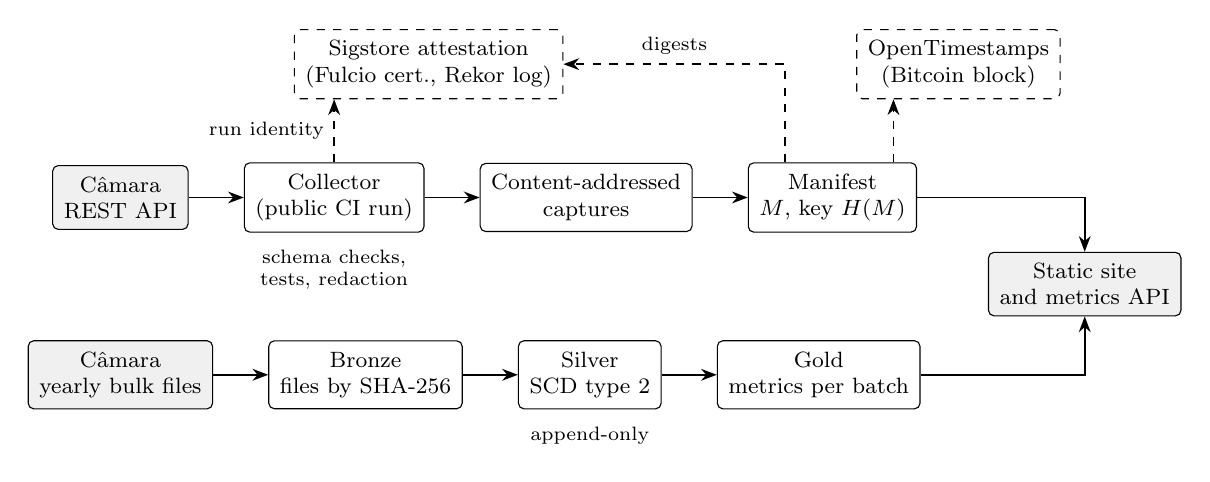
\begin{tikzpicture}[
  font=\footnotesize,
  node distance=5mm and 7mm,
  box/.style={draw, rounded corners=2pt, align=center, inner sep=4pt, minimum height=8mm, fill=white},
  ext/.style={box, fill=black!6},
  proof/.style={box, dashed},
  arr/.style={-{Stealth[length=2mm]}, semithick},
  lbl/.style={font=\scriptsize, align=center}
]
\node[ext] (api) {C\^amara\\REST API};
\node[ext, below=14mm of api] (bulk) {C\^amara\\yearly bulk files};

\node[box, right=of api] (collect) {Collector\\(public CI run)};
\node[box, right=of collect] (cas) {Content-addressed\\captures};
\node[box, right=of cas] (manifest) {Manifest\\$M$, key $H(M)$};

\node[proof, above=8mm of collect, xshift=12mm] (sig) {Sigstore attestation\\(Fulcio cert., Rekor log)};
\node[proof, above=8mm of manifest, xshift=16mm] (ots) {OpenTimestamps\\(Bitcoin block)};

\node[box, right=of bulk] (bronze) {Bronze\\files by SHA-256};
\node[box, right=of bronze] (silver) {Silver\\SCD type 2};
\node[box, right=of silver] (gold) {Gold\\metrics per batch};

\node[ext, right=9mm of manifest, yshift=-11mm] (site) {Static site\\and metrics API};

\draw[arr] (api) -- (collect);
\draw[arr] (collect) -- (cas);
\draw[arr] (cas) -- (manifest);
\draw[arr] (bulk) -- (bronze);
\draw[arr] (bronze) -- (silver);
\draw[arr] (silver) -- (gold);
\draw[arr] (manifest.east) -| (site.north);
\draw[arr] (gold.east) -| (site.south);
\draw[arr, dashed] ([xshift=-3mm]manifest.north east) -- ([xshift=-3mm]manifest.north east |- ots.south);
\draw[arr, dashed] ([xshift=-6mm]manifest.north) |- node[lbl, pos=0.75, above] {digests} (sig.east);
\draw[arr, dashed] (collect.north) -- node[lbl, left] {run identity} (collect.north |- sig.south);

\node[lbl, below=1mm of collect] {schema checks,\\tests, redaction};
\node[lbl, below=1mm of silver] {append-only};
\end{tikzpicture}
\caption{The two data paths. Solid arrows carry data. Dashed arrows carry digests into public infrastructure that the project does not control: a transparency log for the attestation and the Bitcoin blockchain for the timestamp.}
\label{fig:pipeline}
\end{figure}

\subsection{Collection}
\label{sec:collection}

A scheduled workflow on GitHub-hosted runners starts the collector at 09:00 UTC (06:00 in Bras\'ilia) every day. The collector discovers the six bills with the most recent identifiers of the current year and the propositions affected by the eight most recent votings of the month, keeps every proposition collected on earlier days, and refreshes each one's detail, authors, official themes, related votings and individual votes.

The collector treats the source as untrusted input. It accepts only HTTPS URLs on an explicit list of four Chamber hosts, with no port or credentials, and rejects API redirects. Every response is decoded against a schema; a response that does not match stops the run. Two records for the same deputy in the same voting stop the run instead of one being picked silently. Requests time out after 30 seconds and are retried at most twice with exponential backoff and jitter, honouring \texttt{Retry-After}. Output files are written through a temporary file and an atomic rename, and only after the whole collection has validated, so a failed run leaves the previous collection in place.

Two fields are removed from vote captures before anything is stored: each deputy's e-mail address and photo URL. The removal is declared in a \texttt{redactions} list next to the capture, so that a reader does not mistake the capture for a byte-exact HTTP response.

\subsection{Content addressing and the manifest}
\label{sec:manifest}

Each run produces a set of artifacts: one \emph{raw} capture per API response (the URL, the capture time and the decoded body), one \emph{normalized} snapshot that the site renders, and one \emph{legislative} dataset of propositions, votings and ballots. Let $H$ be SHA-256~\citep{fips180-4} and let $c(\cdot)$ be a canonical JSON encoding: object keys sorted recursively by code unit, two-space indentation, one trailing newline. The idea is the same as the JSON Canonicalization Scheme~\citep{rfc8785}, though the encoding is the project's own and is fixed by its source code. Each artifact $x$ of kind $k$ is stored under the key
\[
  \texttt{v1/}k\texttt{/}H(c(x))\texttt{.json},
\]
so equal values always get the same name and the same bytes, and a published object never changes. This is content addressing as used by IPFS and Trusty URIs~\citep{benet2014ipfs,kuhn2014trusty}.

The run's manifest $M$ lists, for every artifact, its kind, key, digest and size, together with the creation time. The manifest is stored under $H(c(M))$. One 64-character string therefore commits to everything the run collected, in the manner of a one-level Merkle tree~\citep{merkle1988signature}. Since $c$ is injective and $M$ contains every artifact's digest, producing a different set of artifacts with the same manifest name would require exhibiting a collision of $H$, either between two manifests or between two artifacts. ``Different'' here means a different canonical encoding: two JSON values that differ only in the order of their keys are deliberately the same artifact. Appendix~\ref{app:lean} proves this reduction.

\subsection{Closing the gap: public code on a public runner}
\label{sec:attestation}

Integrity alone does not answer the sceptical reader's question, because the operator could build a consistent manifest over edited files. The central design decision is therefore about \emph{where} the collector runs.

It does not run on the maintainer's computer or on a server the maintainer rents. It runs on a runner hosted by the CI platform. Each such runner ``is a new virtual machine (VM) hosted by GitHub''~\citep{github-hosted-runners}, created from an image the platform publishes. The maintainer writes the code and the schedule and then has no access to the machine while it works: the platform checks out the public commit, installs the dependencies pinned by the lockfile, runs the collector, the tests and the checks, and produces the files. For public repositories this execution costs the project nothing (``use of the standard GitHub-hosted runners is free and unlimited on public repositories''~\citep{github-runners-reference}), and its logs are public: anyone can open a run and read, line by line, what was executed.

The division of roles is what closes the gap. The maintainer \emph{authors} the collector; the platform \emph{executes} it; a signing service \emph{certifies} which code was executed and what it produced; a public log \emph{records} the certificate; and the result is committed to the repository by the platform's automation account, with a message that names the run. The maintainer never needs to handle a collected data file, and a data file the maintainer did handle is recognisable as such. This holds for the attested files only: the site's pages, the lake and the metrics are built or written outside this path, as the security analysis states.

Open source is the other half. The attestation says ``commit \texttt{ea20c3a} of this repository produced this file''; that sentence is only useful because anyone can read commit \texttt{ea20c3a}. The code is under the MIT licence, its dependencies are fixed by a lockfile, and a reader who distrusts both the maintainer and the platform can fork the repository and run the identical workflow under their own account, as an independent witness.

Concretely, the workflow asks the CI platform to attest the outputs.

After the collector finishes, and only if tests, type checks and formatting checks pass, the workflow calls GitHub's artifact attestation action for three files: the manifest, the legislative dataset and the snapshot. An attestation binds a file digest to an in-toto statement with a SLSA provenance predicate~\citep{torresarias2019intoto,slsa12provenance}. It is signed with a key whose certificate is issued by Sigstore's certificate authority to the workflow's OpenID Connect identity and is valid for ten minutes~\citep{newman2022sigstore,fulcio}; the signature is recorded in the public Rekor transparency log~\citep{github-attestations}. The certificate carries the repository, the workflow file and branch, the commit and the run, and says whether the runner was hosted by GitHub.

Because the manifest is one of the three attested files, the attestation covers every raw capture through its digest. All third-party actions in the workflow are pinned by commit hash, and every package, including the timestamping client and its dependencies, is installed from a frozen lockfile with integrity hashes. This matters because any step in the job could request the signing token: code resolved at run time would be code the attestation does not name. The commit does not fix everything, though: the runner image and the Node.js release are chosen by the platform at run time, and are trusted along with it.

Anyone can repeat the check with the GitHub command-line tool:

\begin{lstlisting}
gh attestation verify legislativo.json -R c0utin/vigiadopovo \
  --signer-workflow c0utin/vigiadopovo/.github/workflows/collect.yml \
  --source-ref refs/heads/main --deny-self-hosted-runners
\end{lstlisting}

The last flag matters. Attestations can also be produced on runners controlled by the repository owner, so a verifier who wants protection from the operator must reject those explicitly. The project's verification guide prescribes exactly this command.

A collection made on a developer's machine records \texttt{collector:\ null} in its provenance file, and the site then states that the collection has no origin attestation.

\subsection{Time: anchoring the manifest in Bitcoin}
\label{sec:time}

The Rekor entry already carries a time, but it is asserted by the same parties that vouch for provenance. For a time bound that depends on none of them, the workflow anchors the manifest in Bitcoin.

The Bitcoin blockchain is used here only as a public, append-only record that nobody controls~\citep{nakamoto2008bitcoin}. About every ten minutes a new \emph{block} is added. Its \emph{header}, 80 bytes long, contains the time at which it was produced, the hash of the previous header, and the root of a Merkle tree over the block's transactions. Thousands of independent nodes keep copies of all headers, and changing an old block would require redoing the proof of work of that block and of every block after it. A digest written into a transaction is therefore fixed in a header that the whole network holds, and the header's position in the chain bounds when it was written. No coins are moved and nothing about the data is revealed: only a 32-byte digest is committed.

The workflow does this through OpenTimestamps~\citep{todd2016opentimestamps}, which makes it free. The client sends the manifest's digest to public calendar servers, which aggregate all digests received in a one-second interval into a Merkle tree and periodically commit a tree of those roots in a single Bitcoin transaction. This follows the linked time-stamping idea of \citet{haber1991timestamp}, with the blockchain as the widely witnessed record.

The receipt is first \emph{pending}: it names the calendar that will complete it. Every later run executes the client's \texttt{upgrade} step on all earlier receipts, which replaces the pending reference with the full path of hash operations from the manifest digest to the Merkle root in a block header. A complete proof needs only the Bitcoin block headers to verify. A calendar cannot attach an existing proof to a different document without finding a collision of a hash function used in the proof, which in practice is SHA-256; at worst it fails to deliver a proof~\citep{todd2016opentimestamps}. The proof is about content, not time: the time bound comes from the block, as explained next.

The proof shows that the manifest existed before the block was mined. Turning that into a date relies on the header's time, which miners set within loose limits: it must exceed the median of the previous eleven blocks and may be up to two hours ahead of network time~\citep{bitcoin-devref-blockchain,szalachowski2018timestamps}. Assuming honest miners, the header time is accurate to within about two hours in either direction, so the proof gives an upper bound on when the manifest existed, with a resolution of hours, and nothing about how long before. Proofs are stored outside the immutable \texttt{v1/} tree, because the upgrade step rewrites them.

\subsection{Why not an on-chain verifier}
\label{sec:onchain}

An obvious alternative is to put the whole check on a programmable blockchain: a contract that verifies, for each collection, a proof that the data came from the Chamber's server, for instance a TLSNotary proof of the HTTPS session or a succinct zero-knowledge proof derived from it, and stores the result. We decided against it for four reasons, of which cost is the first.

\emph{Every verification is paid for, every day, forever.} On Ethereum, checking a pairing-based proof costs 45,000 gas plus 34,000 gas per pairing~\citep{eip1108}, so the pairing check alone of a standard Groth16 verifier, which uses four pairings, costs 181,000 gas; storing each new 32-byte result costs another 20,000 gas, or 22,100 for a slot not yet touched in the transaction~\citep{eip2200,eip2929}. These are gas units, not money; their price in currency varies, but it is never zero, and it recurs with every collection. The system's daily collection, attestation and timestamp cost nothing (goal G8). A design that needs a funded wallet stops the day the wallet is empty, which is exactly the fragility that makes monitoring projects disappear.

\emph{A wallet is a key, and a key is trust.} Paying for transactions requires the project to hold a private signing key, the one kind of secret the data path avoids: the attestations are signed with short-lived certificates issued to the workflow run. The project does hold storage and deployment credentials, which is precisely why the lake and the deployment are not trusted to the same degree. A wallet key would put the operator back in the data path, since whoever holds it decides what is submitted.

\emph{The proof of origin still needs a trusted party.} TLSNotary works by adding a third party, a verifier, which takes part in the TLS connection through secure multi-party computation; its documentation states that the most practical way to use the data on-chain is to prove it to an off-chain verifier, and that ``trust is still required in the designated Verifier when it attests to the verified data on-chain''~\citep{tlsnotary-docs}. An on-chain contract would therefore check the signature of a notary, not the Chamber's server: it would move the trust, not remove it.

\emph{The time guarantee is already available for free.} What a public blockchain adds that nothing else does is a widely witnessed, append-only order of events. OpenTimestamps obtains that property by committing one 32-byte digest per aggregation round, with the cost shared among all users of the calendars and paid by them, not by the project.

The on-chain route is worth revisiting if the Chamber signs its responses, which would remove the notary, or if a public funder wants to pay for a permanent registry. Until then the system uses a blockchain only for what is cheap and necessary: a timestamp.

\subsection{History: an append-only lake}
\label{sec:lake}

The yearly bulk files are rewritten by the Chamber whenever a record of that year changes. A republisher that keeps only the latest copy silently inherits every rewrite. The lake path keeps all of them.

A Rust program downloads four files per year (votings, individual votes, leadership orientations, and the propositions each voting affects) and writes three layers, following the bronze, silver and gold convention of lakehouse systems~\citep{armbrust2021lakehouse}, as Apache Iceberg tables~\citep{iceberg-spec} on object storage. Nothing is updated or deleted; every write is an append.

\emph{Bronze} stores each version of each file exactly as published, once, under its SHA-256, and records per batch the URL, digest, size, collection time and the list of JSON fields the file contained. If the Chamber renames or removes a field the pipeline reads, the year fails with an explicit error instead of filling the column with nulls as though the data had changed.

\emph{Silver} stores typed records as a slowly changing dimension of type~2~\citep{kimball2013toolkit}. A row is one version of one record, identified by a key (for a vote, the voting identifier and the deputy identifier). It carries a content hash, defined as the SHA-256 of the compact JSON array of the record's content columns in table order, an operation code, and the batch in which the version was seen. The operation is \texttt{I} for a new record, \texttt{A} for changed content, and \texttt{R} for a record that left the official file, stored as a tombstone with null content. The state of the record at any instant is its latest version up to that instant. A reader with catalog access can ask what a given vote looked like on a given day.

\emph{Gold} stores the aggregates the site publishes. Each gold row names its \emph{batch}, the SHA-256 of the year's four sorted \texttt{file:sha256} lines. A published metric is thereby tied to the exact bytes of the official files it came from. A year whose files have not changed since the last batch is skipped.

The lake runs as a separate job after the attested collection and cannot block it. Its outputs are not attested; their link to the source is the file digests, which a reader compares against the Chamber's current files.

\subsection{Metrics with public formulas}
\label{sec:metrics}

The site publishes three families of numbers for every year since 2003: votings per month, each deputy's votes by body and position, and the \emph{alignment} of each party with four leaderships that issue voting orientations on most floor votes (Government, Opposition, Majority and Minority).

Let $V=\{\text{Sim},\text{N\~ao},\text{Absten\c{c}\~ao},\text{Obstru\c{c}\~ao}\}$ be the registered positions; absences and the vote of the presiding deputy are outside $V$. Let $\mathcal{V}_{b,a}$ be the individual votes cast in year $a$ in votings where leadership $b$ oriented Sim or N\~ao, and write $\mathrm{orientation}_b(v)$ for that orientation in the voting of vote $v$. For party $p$,
\begin{equation}
\label{eq:alignment}
\mathrm{alignment}(p,b,a)=
\frac{\bigl|\{v\in\mathcal{V}_{b,a} : \mathrm{party}(v)=p,\ \mathrm{vote}(v)\in V,\ \mathrm{vote}(v)=\mathrm{orientation}_b(v)\}\bigr|}
     {\bigl|\{v\in\mathcal{V}_{b,a} : \mathrm{party}(v)=p,\ \mathrm{vote}(v)\in V\}\bigr|}.
\end{equation}
The party is the one registered on each vote, so a deputy who changes party during the year is counted under each. An absence is never counted as a vote. The ratio is undefined when the denominator is zero. The site publishes the numerator and the denominator, not only the ratio. Because the orientation is always Sim or N\~ao, both of which are in $V$, the numerator never exceeds the denominator. Leaderships are identified by their label in the orientation file; the Government leadership appears in the files as both ``GOV.'' and ``Governo'', and the two labels are treated as one. Since orientations are only Sim or N\~ao, an abstention or an obstruction always counts as not coinciding. Appendix~\ref{app:lean} proves that the numerator never exceeds the denominator, that both counts ignore the order of the records and any absences, and that the denominators of all parties add up to the total number of registered votes in the votings the leadership oriented.

The measure is deliberately modest. It is a count of coincidences with a public orientation, close to the roll-call agreement scores long used in the study of Brazilian coalition politics~\citep{figueiredo1999executivo}. It is not an ideal-point estimate~\citep{poole1997congress,clinton2004statistical}, and the site says in each response that coinciding with an orientation does not mean supporting the merit of a bill. The project does not compute each party's alignment with its own leadership, because many parties orient through federations or blocs whose names are truncated in the source, and a join by party label would drop those votes without warning.

The metrics are served by an edge function that executes no query and holds no secret: it validates the year, identifier and leadership against closed lists and returns a slice of a precomputed JSON file. Visitors cannot trigger computation.

\subsection{A deterministic, replayable score}
\label{sec:quality}

The project also implements, but does not publish, a ranking of sitting deputies that scores only outcomes: a bill earns points when the Chamber approves it or when it becomes law, weighted by the kind of norm, reduced for honorific bills and divided among its authors. Filing a bill earns nothing. The scoring function is pure: it reads no clock, network, random source or locale, sorts its input by each bill's identifier, which the Chamber assigns uniquely, before use, and publishes the digests of its exact input and output, so that anyone can replay it and obtain the same bytes~\citep{peng2011reproducible,lamb2022reproducible}. It also reports how each rank moves under alternative weightings. We do not evaluate the ranking here; its risks are discussed with the social impact.

\subsection{Simple language, context and summaries}
\label{sec:plain}

Pages are prerendered and lead with the answer: what was voted, who voted how. Reading a bill page, the method page or the transparency page requires no JavaScript. The site describes itself as explaining the Chamber in \emph{linguagem simples}, the term of the national policy~\citep{brasil2025lei15263}: short sentences, common words and the most important information first. Each vote is shown with its context: the bill it concerns, its official summary and the result, and, on the metrics pages, how each party has voted relative to the leaderships' orientations over the years. Each bill shows the official summary (\emph{ementa}) and, when one exists, a short explanation in simple language generated by a language model.

Generated text is the part of the site that cannot be verified, so it is fenced. A summary covers only the official summary text, never the full bill. It is bound to its source by the SHA-256 of the pair (bill identifier, official summary): if the Chamber changes the summary, the hash no longer matches, the explanation is withdrawn and the bill returns to a queue. Each explanation is labelled as machine-generated and not reviewed by a person. The explanations reach the collector as a file that the maintainer commits, so the label is the operator's declaration: the attestation proves which explanations were published, not who or what wrote them. No model produces any number on the site.

The site also offers its content as plain text (an index file and Markdown versions of its pages) for readers who use AI assistants, on the reasoning that a model answering a question about a vote should be handed the official record and its caveats instead of recalling them.

\subsection{Deployment and cost}
\label{sec:deploy}

The site is a static bundle served from a CDN's free tier. The collection, attestation and timestamping run on free CI minutes for public repositories. The lake uses an object store's free allowance; before any write, a budget check reads the month's real usage from the provider's analytics API and stops the job when any allowance reaches 80\%. Visitor traffic cannot create a bill. Static pages do not invoke the edge function; the function is capped by its free plan at 100,000 requests a day, after which requests fail; and it reads the object store at most twice per request (once, except in early January, when a request without a year falls back to the previous year), which bounds reads at about 3.1 million a month against an allowance of 10 million.

\section{Implementation}
\label{sec:impl}

The system is small enough for one person to read in a few days, which is part of its security argument: the attestation names the code that ran, and that is useful only if someone can read it. Table~\ref{tab:software} lists its parts.

\begin{table}[t]
\centering
\small
\begin{tabularx}{\textwidth}{@{}>{\raggedright\arraybackslash}p{3.6cm}>{\raggedright\arraybackslash}p{5.0cm}>{\raggedright\arraybackslash}X@{}}
\toprule
Part & Technology & Runs on \\
\midrule
Collector, pipeline, metrics publisher, edge function & TypeScript on Node.js, with the Effect library & CI runner; edge function on the CDN \\
\addlinespace[3pt]
Lake & Rust, Polars, Apache Iceberg & CI runner; tables in object storage \\
\addlinespace[3pt]
Site & Svelte~5 and SvelteKit, prerendered to static files & CDN \\
\addlinespace[3pt]
Tests & Node.js test runner; Rust unit tests & CI runner \\
\bottomrule
\end{tabularx}
\caption{The parts of the software.}
\label{tab:software}
\end{table}

\emph{Collector and pipeline.} The collector is written as typed effect programs. Every response from the Chamber is decoded against a schema before use, expected failures travel in a typed error channel, and network, clock and file system are injected dependencies, so the tests replace the network with fixtures and exercise timeouts, retries, malformed responses and duplicated votes without credentials or paid services. Data transformations are pure functions; input and output happen at the edges. Published files are always written through a temporary file and an atomic rename.

\emph{Lake.} A single Rust binary downloads the yearly files, checks their field lists, builds typed tables with a dataframe library, computes the type-2 differences against the stored state and appends them as Iceberg snapshots. The same binary can write plain Parquet files to a local folder with no cloud account, so the whole lake can be rebuilt on a laptop from the Chamber's files.

\emph{Site.} Pages are prerendered at build time and served as static files; there is no server-side rendering, database or session at request time. The site offers: recent bills with their official summaries and explanations in simple language; a page per bill with its votings; an explorer of individual votes filterable by theme, bill, deputy, party, state and position; a list and a profile page for each of the 513 sitting deputies, and the roster of every legislature since 1826; the yearly metrics since 2003; a transparency page that lists the artifacts and proofs of the current collection; and plain-text versions of its content for AI assistants. A build step enforces transfer budgets, for example at most 14\,KiB of compressed HTML and no JavaScript modules on the home page.

\emph{Edge function.} The only code that runs per request serves \texttt{/api/metricas}. It validates parameters against closed lists, reads precomputed JSON from storage behind two layers of cache, at most twice per request, and holds no secret.

\emph{Tests and release gate.} JavaScript and Rust tests cover the collection contract, the failure modes, the determinism of the scoring function under permutation of its input, the edge function's validation and caching, and the storage-allowance check. Deployment is a single script that refuses to run unless the working tree is clean and identical to the main branch on both remotes, then runs formatting, tests, type checks, a dependency audit, the build and the page-size budget check, writes a checksum of every published file, and deploys.

\emph{Engineering rules.} The contribution guide forbids hand-edited output files, compatibility shims and unreviewed claims of human review, and requires that every source be official. These are social rules, not proofs, but they are the rules that the attested workflow enforces mechanically for the data path.

\section{Security analysis}
\label{sec:security}

Table~\ref{tab:claims} lists each claim a reader may want to check, the mechanism that supports it, and what still has to be trusted. The rest of this section argues each row and then states what the system does not prove.

\begin{table}[t]
\centering
\small
\begin{tabularx}{\textwidth}{@{}>{\raggedright\arraybackslash}p{3.6cm}>{\raggedright\arraybackslash}p{3.9cm}>{\raggedright\arraybackslash}X@{}}
\toprule
Claim & Mechanism & Still trusted \\
\midrule
A file was not changed after collection & SHA-256 in the manifest and in the file name & Nothing beyond SHA-256, once the manifest is authenticated \\
\addlinespace[3pt]
A file was produced by the public collector at a given commit and run & Sigstore attestation of the manifest and data files & The CI platform, its hosted runners, runner image and Node.js release; Sigstore's certificate authority and log \\
\addlinespace[3pt]
The collection existed by a given time & OpenTimestamps proof ending in a Bitcoin block header & Bitcoin's proof of work; honest header times (about two hours); block explorers, unless the reader runs a node \\
\addlinespace[3pt]
An official record was later changed or removed & Append-only versions with content hashes & The lake operator, for versions the Chamber no longer serves \\
\addlinespace[3pt]
A metric follows from the official files & Public formula; digests of the source files & The Chamber's current files and the reader's reading of the formula, while the Chamber still serves the same files \\
\addlinespace[3pt]
The deployed site is the one that was built & \texttt{SHA256SUMS} written at each deploy & The deployer: the list is not attested \\
\addlinespace[3pt]
The site shows the latest collection & None: the site is deployed by hand & The operator and the deployer; the reader's comparison with the list of attested runs \\
\addlinespace[3pt]
The Chamber returned this content & None: the API does not sign its answers & TLS at collection time; comparison with the live API \\
\addlinespace[3pt]
A simple-language summary is correct & None: unreviewed text, supplied by the operator and labelled as model output & The operator; the reader's comparison with the official text \\

\bottomrule
\end{tabularx}
\caption{What each proof establishes and what remains trusted.}
\label{tab:claims}
\end{table}

\subsection{Integrity}

Suppose the manifest name $h_M$ is known to be authentic. To replace an artifact $x$ with $x'\neq x$ under the same key, the operator, the host or a network attacker must find a second preimage of $H$, which for SHA-256 has an expected strength of 256 bits for short messages and never less than 201 bits for the longest ones~\citep{sp800-107r1,kelsey2005second}. By the length-dependent bound, the largest artifact in a manifest (237\,kB) keeps about 244 bits and the largest bulk file in the lake (198\,MB) about 234 bits. The integrity argument does not depend on the transport, so it holds against the host and the network as well as the operator.

Collision resistance (128 bits for SHA-256~\citep{sp800-107r1,rogaway2004hash}) is the relevant property only for a party that chooses both colliding files \emph{before} publication. That party is the operator. A collision would let the operator obtain one attestation and one timestamp covering two different collections and later show whichever suits. No such attack on SHA-256 is known; the full collision on SHA-1~\citep{stevens2017sha1} shows why the choice of function matters. Known quantum algorithms lower the query bounds to about $2^{128}$ for preimages~\citep{grover1996search} and about $2^{85}$ for collisions~\citep{brassard1998quantum}, and NIST expects hash functions of this size to remain usable~\citep{nistir8105}.

\subsection{Provenance}

A valid attestation shows that a workflow run holding the stated identity signed a statement about a file with that digest, and that the signature was logged~\citep{github-attestations}. With the verification flags given earlier, the identity is the public collection workflow on the main branch, on a runner hosted by the platform.

This defeats the operator in the role that matters most. To publish an edited file with a valid attestation, the operator would have to commit code that performs the edit to the public repository, where the commit is visible and named in the certificate. Hand-editing an output and committing it is detectable: the file no longer matches any attested digest. The evaluation confirms this.

The guarantee has stated limits. GitHub describes attestations alone as meeting SLSA Build Level~2~\citep{github-attestations}, the level at which forging provenance ``requires an explicit `attack', though this may be easy to perform''~\citep{slsa12}. Only the certificate fields and the log timestamp are outside the control of the workflow that produced the attestation; an attacker inside the run could falsify the rest of the predicate~\citep{gh-attestation-verify}. The platform itself warns that attestations ``are not a guarantee that an artifact is secure''~\citep{github-attestations}. In our setting this means: the attestation proves which public code ran, and proves nothing about whether that code is correct or whether its input was authentic. A reader must still read the collector, or trust someone who has. The collector's own code is short, about a thousand lines, but the code that ran also includes its dependencies, fixed by the lockfile, and the runner image. And the verification command accepts any commit on the main branch: it shows that the public collector produced the file, not that the version which ran had been reviewed. A verifier who wants more can pin the expected commit, or the project can tag reviewed releases and attest only from them.

The operator also controls the repository and could, in principle, push a malicious commit, let it run once, and force-push it away. The certificate and the public log entry would still name the commit hash, but the code would be harder to obtain. The platform often keeps force-pushed commits retrievable by their hash for some time, but does not promise to. Independent forks that mirror the repository, and archives that copy it (Section~\ref{sec:freshness}), remove this weakness.

\subsection{Time}

A complete proof shows that $h_M$ was committed in a block at a given height. Rewriting it would require redoing the proof of work of that block and all later ones~\citep{nakamoto2008bitcoin}. The time claim is an upper bound with a precision of hours; it says nothing about how long before the block the data existed. The attestation's log entry gives a second time, asserted by the signing service; for the manifest of 9 November it is 26 seconds after the manifest's creation, and the attesting block's header time 47 minutes after it (Section~\ref{sec:eval-time}).

What the timestamp adds over the transparency log is independence. It survives the disappearance of the repository, the CI platform, the signing service and the project itself: the proof file and the manifest are enough, with any copy of the block headers. Provided that someone keeps the manifest, the files and the proof, a reader ten years from now can still show that the collector had recorded a given record of a given vote by November 2026. That proviso is the subject of the next subsections.

\subsection{Immutability: how the stored data is kept from changing}
\label{sec:immutability}

``The database'' is three stores with different guarantees. For each we separate what \emph{prevents} a change, what would \emph{detect} one, and what is left to trust.

\emph{The collection archive (git).} Raw captures, snapshots and manifests are files in the public repository, under names that are their own SHA-256 digests. Three things protect them. A file cannot be altered in place without its name ceasing to match its content, which any reader can test with one command. The repository's history is itself a chain of hashes: each commit commits to the full tree and to its parent, so rewriting an old collection changes every later commit identifier, in a repository that is public and that any reader can clone and keep. And the manifest of each collection is attested and timestamped outside the repository, so even a rewritten history could not produce a different manifest carrying the old attestation or the old Bitcoin proof. We checked the history directly: across all commits, no file under the immutable archive path has ever been modified or deleted.

\emph{The lake (object storage).} The lake is append-only by construction. Its program contains no update and no delete: a raw official file is written only if no object with that digest exists, and tables grow only by appending new data files in a new table snapshot~\citep{iceberg-spec}. A correction by the Chamber does not replace a row; it adds a version. Three digests make the content checkable from outside: the object name of each raw file is its SHA-256; each silver row carries a hash that anyone can recompute from that raw file; and each batch identifier is the hash of the year's four file digests, published with every metric. The evaluation uses exactly these to confirm that the published figures match the Chamber's current files.

Here the guarantee is weaker than for the archive, and we say so plainly. Append-only is a property of the program, not of the storage: whoever holds the storage credentials could delete or replace objects. On the day of our measurements the bucket had no retention lock configured. The lake's batches are not attested or timestamped, so for versions that the Chamber no longer serves, the lake is the only witness. A reader can always detect a lake that disagrees with the Chamber's current files; a reader cannot yet prove what the lake said last month.

Two inexpensive measures would close most of this. The storage provider offers bucket locks that ``prevent the deletion and overwriting of objects''~\citep{cloudflare-bucketlocks}; a lock on the raw-file prefix would turn append-only from a convention into an enforced rule against accident and against a leaked write key, though not against the account owner, who can remove the rule. And the workflow could compute a running digest of the lake, $h_n = H(h_{n-1} \,\|\, b_n)$ over successive batch identifiers $b_n$, with $h_0$ a fixed constant such as 32 zero bytes and $\|$ the concatenation of the 32-byte $h_{n-1}$ with $b_n$, and attest and timestamp $h_n$ each day alongside the manifest. Any later rewrite of an old batch would then contradict a value already anchored in a public log and in the Bitcoin blockchain. This is the construction of tamper-evident logs~\citep{crosby2009tamper}, applied with the tools the project already uses; Appendix~\ref{app:lean} proves that a rewrite which keeps the number of batches yields a collision of $H$, and that one which adds or removes batches yields a collision of $H$ or a preimage of $h_0$; a counterexample shows the second case cannot be dropped.

\emph{The published metrics.} The JSON files served by the API are derived data and are replaced whenever a year's batch changes. Their protection is not immutability but reproducibility: each carries its batch identifier and the digests of its source files, and can be regenerated from them.

In short: the collection archive is protected by naming, public history and external anchors; the lake by construction and by recomputation, with enforcement and anchoring still to be added; and the metrics by being recomputable.

\subsection{Freshness, hidden inputs and preservation}
\label{sec:freshness}

\emph{Freshness and rollback.} The proofs show that a collection is authentic, not that it is the latest. A host, or the operator, could serve an older manifest that still verifies; during our measurements the site's transparency page named a manifest of 9 November although later collections existed. Nothing in the design stops the operator from running the workflow several times and publishing the result that suits, either: there are three collections for 8 November. The defence is that every run and every attestation is public, so a reader can list all collections and compare the one served with the newest. Two cheap measures make this routine: the site should show the newest manifest and its time on every page, and the verification guide now asks the verifier to compare the served manifest with the newest one on the main branch and to report the trigger of the run.

\emph{Hidden inputs.} The attestation names the commit, but a run also depends on inputs that are not in the commit. The collection job uses no secret, but it restores a dependency cache from earlier runs and can be started by hand as well as by the schedule. The certificate records the trigger, so a verifier can require scheduled runs only; the cache is trusted to match the lockfile. Some inputs that are in the commit are data, not code: the collector reads the list of propositions from the previous snapshot in the repository and refreshes each one, so a commit that edits that list changes what the next attested collection covers. Such an edit is a public commit, and the verification guide asks the verifier to list commits by people that touched the data files; up to the measurements none had since the first attested collection of 5 November; the guarantee is that every human influence on a collection is public, not that there is none. The generated summaries are written outside the workflow and committed as an input file: the attestation shows which summaries were published, not how they were produced. The lake job, which holds the storage credentials, is not attested at all.

\emph{Preservation.} A timestamp outlives the project only if someone keeps the manifest, the files and the proof. The CI platform deletes run logs and artifacts after a retention period~\citep{github-log-retention}, and the repository can be deleted by its owner. Universal source archives such as Software Heritage~\citep{dicosmo2017software} preserve public repositories with their full history under intrinsic hash identifiers, and would keep the archive, the proofs and the code that produced them beyond the life of the project. Requesting such archival after each collection would turn the ten-year claim from a possibility into a plan. Since 20 November the workflow also stores each collection's attestation bundle next to its timestamp proof, so the bundle no longer depends on the platform's retention, and a verifier need not fetch it from the platform's API, which is what the evaluation below used a GitHub account for.

\subsection{What is not proven}
\label{sec:notproven}

\emph{Origin.} The Chamber's API does not sign its responses. The collector authenticates the server by TLS when it connects, but TLS leaves no transferable evidence: a third party cannot later check that the bytes came from the Chamber. Everything downstream is therefore a proof about what the collector \emph{recorded}, not about what the Chamber \emph{said}. \citet{lemieux2016trusting} draws the same line for blockchain record keeping in general: such systems protect the integrity of what was registered, not the reliability of the record at its creation.

Three things narrow this gap without closing it. A reader can fetch the same URL today and compare fields, since each raw capture stores its URL and capture time. Anyone can run the same workflow from a fork as an independent witness; two unrelated collectors recording the same content at the same time would be much harder to explain away. Their manifests will never be byte-identical, because each capture embeds its own capture time, so witnesses must be compared record by record on the decoded response bodies, ignoring the capture metadata. And for the bulk files, the lake records a digest that a reader can compare with the file the Chamber serves now.

The gap could be closed from either side. The Chamber could sign its responses, for instance with HTTP Message Signatures~\citep{rfc9421} under a certificate of the national public-key infrastructure~\citep{mp2200-2}. Failing that, a collector could produce a transferable proof of the TLS session with a protocol such as DECO or TLSNotary~\citep{zhang2020deco,tlsnotary}, at the cost of a third-party notary and a much heavier client.

\emph{Deployment.} The site is built and deployed from the maintainer's environment, not from CI. The deploy writes a checksum of every published file, but that list is not attested, so it shows that the site is internally consistent, not who built it. The attested data files can be checked directly; the HTML that presents them cannot, except by rebuilding the site from the public source.

\emph{Deputy profiles and metrics.} Profile files are attested by a separate monthly workflow and are not part of the manifest. The lake's tables and the metrics derived from them are not attested at all; they rest on recomputation from the Chamber's files.

\emph{Completeness.} Nothing proves that the collector recorded \emph{every} relevant record. A collector that systematically skipped a class of votes would produce valid proofs. The defence is again public code and recomputation of totals.

\emph{Summaries.} No mechanism checks that a generated explanation is faithful to the text it explains.

\section{Evaluation}
\label{sec:eval}

We evaluate the deployed system, not a prototype. All measurements were taken on 16 November 2026 against the public site and the public repository, using only public data: the site, the Chamber's servers, the repository, its attestations and CI logs, and public Bitcoin block explorers. We ask whether the proofs verify, whether the published numbers can be recomputed without the project's code, whether the source changes underneath the republisher, what operation costs, and whether the numbers are plausible. The system had been running for only a few weeks, so the evaluation shows that the mechanisms work, not that they survive years of operation.

\subsection{Following the public verification guide}
\label{sec:eval-verify}

The repository ships a verification guide. We followed its steps against the live site, using only public data, although with a client signed in to the first author's own GitHub account, which the command-line tool requires. The first author ran every check in this section, with the AI assistant credited at the end of the paper, which also helped write the project's code; the checks are therefore a demonstration that the mechanisms work, and an independent repetition remains to be done.

\emph{Finding the collection.} The transparency page named manifest \texttt{0290c5d7\ldots7d4c}, created on 9 November 2026 at 19:43:28 UTC, listing 254 artifacts.

\emph{Provenance.} \texttt{gh attestation verify}, with the flags given in the design, succeeded for the manifest, the legislative dataset and the snapshot served by the site. The verified certificate named the issuer \texttt{token.actions.githubusercontent.com}, the signer \texttt{collect.yml@refs/heads/main}, the trigger \texttt{schedule}, the commit \texttt{ea20c3a}, a specific run, and a GitHub-hosted runner; the predicate type was SLSA provenance v1; and the transparency-log timestamp was 19:43:54 UTC, 26 seconds after the manifest was created. The deputy-profile file verified in the same way against the monthly workflow.

\emph{Integrity.} The manifest hashed to its own name. We downloaded all 254 artifacts from the site (952,233 bytes) and recomputed each digest: 254 matched and none differed.

\emph{Time.} The OpenTimestamps client reported that Bitcoin block 975,215 attests the manifest's existence as of 9 November 2026.

\emph{A tampered file.} We flipped one bit inside the official summary of the first bill in the snapshot file and repeated the provenance check. Verification failed: no attestation exists for the altered digest. This outcome follows from the construction, and the test only confirms that the verification command rejects it as designed; an operator who edits a published file by hand cannot keep the attestation. The attacks that would test the design itself, attesting from a self-hosted runner, from a branch or from a commit later force-pushed away, were not attempted.

The full check took a few minutes, most of it spent downloading the 254 artifacts one at a time. It needs a command line, the GitHub client with an account, and a JavaScript runtime. That is a real barrier, to which we return when discussing who can verify.

\subsection{Timestamps}
\label{sec:eval-time}

The repository held 13 manifests. Twelve had a timestamp proof; the one without is the earliest, created within an hour of the repository. Eleven proofs in the repository were complete; the newest was still pending, and the client completed it from a calendar server during verification. All twelve then verified against a Bitcoin block (Table~\ref{tab:timestamps}). We verified with the client's light mode, which takes block headers from public block explorers; a reader who wants no such dependency needs a Bitcoin node.

\begin{table}[t]
\centering
\small
\begin{tabular}{@{}llrrr@{}}
\toprule
Manifest & Created (UTC) & Artifacts & Block height & Delay (min) \\
\midrule
\texttt{bafb55d2} & 30 Oct 00:26 & 83  & 974,448 & 7,090 \\
\texttt{218fd2c5} & 05 Nov 17:16 & 162 & 974,697 & 128 \\
\texttt{deb9d8a9} & 06 Nov 16:42 & 238 & 974,832 & 49 \\
\texttt{65f9a1b4} & 07 Nov 15:35 & 238 & 974,951 & 66 \\
\texttt{f49da990} & 08 Nov 15:53 & 238 & 975,079 & 52 \\
\texttt{1994f262} & 08 Nov 18:11 & 238 & 975,091 & 84 \\
\texttt{4e5ead96} & 08 Nov 18:59 & 238 & 975,091 & 37 \\
\texttt{0290c5d7} & 09 Nov 19:43 & 254 & 975,215 & 47 \\
\texttt{aa8a1def} & 12 Nov 17:30 & 372 & 975,582 & 92 \\
\texttt{9298a345} & 13 Nov 17:06 & 396 & 975,705 & 157 \\
\texttt{0c63fc5e} & 14 Nov 15:43 & 416 & 975,819 & 74 \\
\texttt{05513dea} & 15 Nov 16:13 & 416 & 975,985 & 10 \\
\bottomrule
\end{tabular}
\caption{The twelve timestamp proofs in the repository, all verified on 16 November 2026. Delay is the time from the manifest's creation to the header time of the attesting block. The first manifest was made on a developer's machine before the workflow existed, carries no attestation, and was stamped almost five days after its creation. Two manifests of 8 November share a block.}
\label{tab:timestamps}
\end{table}

For the eleven manifests stamped in the run that created them, the attesting block's header time followed the manifest's creation by a median of 66 minutes (minimum 10, maximum 157). Block header times are themselves only accurate to within about two hours, so these figures describe the order of magnitude: a collection is anchored within one to three hours. Between collection and the next day's upgrade step, the published proof is pending and its verification depends on the calendar servers being reachable.

\subsection{Recomputing published numbers without the project's code}
\label{sec:eval-recompute}

The strongest check of a number is to compute it again by other means. We wrote a script of about 60 lines in plain Python, using only the standard library and sharing no code with the project (whose aggregation is written in Rust on a dataframe library); it is published as \texttt{docs/paper/scripts/recompute.py}. Its author is the project's author, the first author of this paper, so it shares his reading of Equation~\ref{eq:alignment} and checks the implementation against that reading, not the reading itself. The script downloads the Chamber's yearly files of individual votes and leadership orientations, applies Equation~\ref{eq:alignment}, and compares the result with the site's API row by row. We ran it for four years chosen to span the series (2011, 2019, 2023 and 2026) and all four leaderships. It also asserts that no voting has two Sim or N\~ao orientations from the same leadership, which Equation~\ref{eq:alignment} assumes and a join of votes with orientations would otherwise double-count; the assertion held in every year, and the lake now checks the same condition.

\begin{table}[t]
\centering
\small
\begin{tabular}{@{}lrrrrr@{}}
\toprule
Year & Vote records & Party rows compared & Rows that differ & Source files & Digests equal \\
\midrule
2011 & 33,235  & 48  & 0 & 2 & 2 \\
2019 & 120,998 & 138 & 0 & 2 & 2 \\
2023 & 128,679 & 89  & 0 & 2 & 2 \\
2026 & 53,177  & 88  & 0 & 2 & 2 \\
\midrule
Total & 336,089 & 363 & 0 & 8 & 8 \\
\bottomrule
\end{tabular}
\caption{Independent recomputation of the alignment metric from the Chamber's files. A party row is one (party, leadership) pair with its two counts. In 2011 the files contain no Sim or N\~ao orientation for two of the four leaderships, and the site likewise publishes no rows for them.}
\label{tab:recompute}
\end{table}

All 363 published rows matched exactly, in both the numerator and the denominator (Table~\ref{tab:recompute}). For the Government leadership in 2019, for example, both computations give 95,133 registered votes of which 72,537 coincide with the orientation.

The script also hashed the eight files it downloaded and compared them with the digests the project publishes for the same year. All eight were equal, including six that the project had recorded eleven days earlier. A reader can therefore confirm, today, that the metrics were computed from the same bytes the Chamber is still serving.

The digests proved useful in an unplanned way. On our first attempt, several downloads from the Chamber's server were cut short, and the digest comparison was the first check to flag a truncated file.

\subsection{The source changes}
\label{sec:eval-drift}

The lake's logs from its successful daily runs between 8 and 16 November show how the current year's files move. In one run the four files were byte-identical to the previous batch and nothing was written. In three runs new records arrived (in the largest, 602 votings and 492 voting--proposition links). In two runs records that already existed were rewritten in place: one voting on 8 November and five voting--proposition links on 16 November. No record was removed.

Six records rewritten in place, in two runs over nine days, is a small number, and each rewrite is probably a routine correction. The point is that they happen without notice, in files whose names do not change. A republisher that overwrites its copy cannot say what a record looked like last week; the versioned tables can.

\subsection{Operation and cost}
\label{sec:eval-ops}

Between its first run on 5 November and the measurements, the workflow ran 13 times: 11 on its schedule and two started by hand on 8 November. The collection succeeded in 11 runs, each of which produced one of the manifests of Table~\ref{tab:timestamps}, and failed in two, on 10 and 11 November; the lake job failed at its budget check in the first five runs and succeeded in every later run in which it started. Failures were closed. On the two days when the collection step failed, no manifest was written and the previous collection stayed in place; a transparency tool that publishes a partial collection as though it were complete would be worse than one that publishes nothing that day. Scheduled runs set for 09:00 UTC started six to eleven hours late: the CI platform does not guarantee start times for scheduled workflows, and a project that depends on free CI inherits that. A collection run took a median of 2.6 minutes, and a lake run about two minutes.

The complete history from 2003 to 2026, as 96 source files totalling 1.52\,GB of JSON, occupies 244\,MB in object storage, 2.4\% of the free allowance. Every other monthly allowance was at or below 0.3\%. The system has cost nothing to run.

On reach, the home page's HTML weighs 12.1\,kB compressed, and the transparency page (23.0\,kB) contains no script element. The build fails if a page exceeds its byte budget. These are transfer sizes computed from the build, not measurements on real phones.

\subsection{Face validity of the alignment metric}
\label{sec:eval-face}

The lake covers 177,319 votings from 2003 to 2026, of which 26,331 took place on the floor and 6,051 have individual vote records in the official files. Over the whole period, 1,496,140 registered votes were cast in votings where the Government leadership oriented Sim or N\~ao, and 73.6\% of them coincided with the orientation. For the Opposition leadership, which appears in the files from 2018, the figure is 53.1\% of 721,115.

\begin{figure}[t]
\centering
\begin{tikzpicture}
\begin{axis}[
  width=0.96\textwidth, height=6.2cm,
  xmin=2002.5, xmax=2026.5, ymin=0, ymax=100,
  xtick={2003,2005,...,2025},
  x tick label style={/pgf/number format/1000 sep=, font=\footnotesize},
  y tick label style={font=\footnotesize},
  ylabel={\footnotesize Votes coinciding with the Government orientation (\%)},
  ylabel style={align=center, text width=5.5cm},
  ymajorgrids, grid style={black!10},
  legend style={font=\footnotesize, at={(0.5,1.03)}, anchor=south, legend columns=4, draw=none, /tikz/every even column/.append style={column sep=3mm}},
  unbounded coords=jump,
  every axis plot/.append style={thick, mark size=1.3pt},
]
\draw[black!35, dashed] (axis cs:2015.5,0) -- (axis cs:2015.5,100);
\draw[black!35, dashed] (axis cs:2018.5,0) -- (axis cs:2018.5,100);
\draw[black!35, dashed] (axis cs:2022.5,0) -- (axis cs:2022.5,100);
\node[font=\scriptsize, black!60, anchor=south] at (axis cs:2009,1) {PT presidents};
\node[font=\scriptsize, black!60, anchor=south] at (axis cs:2017,44) {Temer};
\node[font=\scriptsize, black!60, anchor=south] at (axis cs:2020.5,44) {Bolsonaro};
\node[font=\scriptsize, black!60, anchor=south] at (axis cs:2024.5,1) {Lula};
\addplot[black, mark=*] table[x=year, y=PT] {data/alignment.dat};
\addplot[black!55, mark=square*, densely dashed] table[x=year, y=PSDB] {data/alignment.dat};
\addplot[black!55, mark=triangle*, densely dotted] table[x=year, y=PSOL] {data/alignment.dat};
\addplot[black!30, line width=2.2pt, mark=none] table[x=year, y=all] {data/alignment.dat};
\legend{PT, PSDB, PSOL, All parties}
\end{axis}
\end{tikzpicture}
\caption{Share of each party's registered votes that coincide with the Government leadership's orientation, by year, as published by the site (Equation~\ref{eq:alignment}). Parties are the labels registered on each vote. Dashed lines separate presidencies; 2016 mixes the last months of Dilma Rousseff's government with the first of Michel Temer's.}
\label{fig:alignment}
\end{figure}

Figure~\ref{fig:alignment} plots the metric for three parties whose labels are stable over the period. The series reproduces what any observer of Brazilian politics knows, which is the purpose of a face-validity check. The PT coincides with the Government orientation in 87\% to 99\% of its votes while it holds the presidency (2003 to 2015 and 2023 to 2026), and in 11\% to 27\% under Temer and Bolsonaro (2017 to 2022). The PSDB moves the other way: between 14.5\% and 61\% under PT presidents until 2015, and between 79\% and 95\% from 2016 to 2022. The PSOL, a smaller left-wing party, ranges from 26\% to 67\% before 2016, falls to between 5\% and 20\% from 2017 to 2022, and reaches 78\% to 91\% under the current government.

The aggregate line carries a second known fact. Across all parties, coincidence with the Government never falls below 64.8\% in any year, the pattern of large, heterogeneous governing coalitions that the literature calls coalition presidentialism~\citep{abranches1988presidencialismo,limongi1998bases}. Its two lowest points are 2015 (64.8\%), the year before Rousseff was removed from office, and 2025 (66.9\%).

We do not claim these observations as findings; the metric's simplicity limits what it can support. Roll calls are also a selected sample: only 6,051 of the 177,319 votings have individual vote records, and recorded votes are known to differ systematically from unrecorded ones, which can bias any analysis built on them~\citep{carrubba2006off,hug2010selection}. We claim only that numbers a citizen can recompute from official files tell a story that is consistent with the scholarly record.

\section{Social impact: what verifiability can and cannot do}
\label{sec:discussion}

It would be easy to end a paper like this with the claim that cryptographic proofs restore trust in politics. The evidence does not support that claim, and this section tries to state the expected impact with the same care as the security claims.

\subsection{What changes}

\emph{The question changes from ``whom do you believe?'' to ``did you check?''.} When two people disagree about how a party voted, a conventional site offers its reputation. This one offers a procedure: the official files, their digests, a formula, and a count that either reproduces or does not. The procedure gives the same answer to a supporter of either side. In a polarised country where each side assumes the other's sources are captured, a number that does not depend on a source's good faith is a different kind of object.

\emph{An edit leaves evidence.} The common suspicion about a politically sensitive site is that someone will quietly adjust it. Here a quiet adjustment is detectable by anyone, as the tamper test showed, and the published history shows when the official record itself changed. For the attested data, the operator's honesty stops being an assumption and becomes an observable; the pages that present it are still built by the operator.

\emph{The record outlives the project.} Monitoring organisations close and their archives vanish. A manifest and its timestamp proof remain verifiable with no surviving party.

\emph{The source is put on the spot.} Once every later step is provable, the one unproven step is conspicuous: the Chamber does not sign what it publishes. The declaration of parliamentary monitoring organisations already asks parliaments to ``guarantee that the information [they release] to the public is accurate''~\citep{openingparliament2012declaration}. Signed responses are a small technical measure with which a legislature could meet that request, and a design like ours shows what it would enable.

\subsection{What does not change}

\emph{Information alone rarely changes votes.} The largest coordinated test of the idea, six randomised trials in five countries including Brazil, found ``no evidence overall that typical, nonpartisan voter information campaigns shape voter behavior''; the pooled effect on the incumbent's vote was statistically indistinguishable from zero for both good and bad news~\citep{dunning2019metaketa}. In the Brazilian trial, voters strongly sanctioned malfeasant mayors in hypothetical scenarios and took no action when given the same information about their own mayor~\citep{boas2019norms}. The closest experiment to a legislator scorecard, covering every member of Uganda's parliament, found no change in members' behaviour and no effect on re-election; only one voter in eight had heard of the scorecard~\citep{humphreys2012policing}.

\emph{Where disclosure did matter, an intermediary carried it.} The release of municipal audits in Brazil reduced the re-election of mayors with reported violations, and the effect was larger where local radio existed to spread the findings~\citep{ferraz2008exposing}. In the United States, members of Congress who receive less local press coverage work less for their constituencies~\citep{snyder2010press}. Transparency produces accountability only through actors able to use it and sanctions able to follow it~\citep{fox2007uncertain,fung2007full,peixoto2016when}.

\emph{Disclosure can also harm.} Corruption information lowered turnout in Mexico: voters withdrew instead of sanctioning~\citep{chong2015corruption}. Transparency experiments have found weak and sometimes negative effects on trust in government~\citep{grimmelikhuijsen2013effect}. \citet{lessig2009against} warned that raw legislative data invites spurious readings that an inattentive audience cannot correct, and that the result is cynicism. A country in which two voters in three cannot name a deputy is exposed to exactly that.

\emph{Proofs do not persuade people who believe a falsehood.} The correction literature reviewed earlier gives no reason to think that a digest will move someone whom a fact-check did not.

From this evidence we draw a modest theory of change. The realistic users of verifiable legislative data are not the median voter but the intermediaries who reach voters: journalists, fact-checkers, teachers, researchers, advocacy groups and, increasingly, AI assistants. For them, a figure that can be cited with a proof is cheaper to use and harder to attack. Whether this improves what reaches citizens is an empirical question that this paper does not answer.

We are also unable to measure it. The site uses no analytics, no cookies and no accounts, as a matter of privacy; the hosting platform keeps short-lived request logs for the metrics API, for debugging, which we did not analyse. We therefore have no data on who uses the site or how. We report no usage figures because none exist.

\subsection{Who can verify}
\label{sec:whoverifies}

``Anyone can verify'' is true in the sense that no permission is needed. In practice, the verification we carried out needs a command line, a GitHub account and familiarity with digests, in a country where 29\% of adults are functionally illiterate~\citep{inaf2024} and a sixth of the population is offline~\citep{carro2026brazil}. Verifiability is exercised by a few on behalf of the many, as with open-source software and published science. Its value to the many depends on the few existing, being independent, and being heard.

The project takes one unusual step to widen that group. Its verification guide is written for AI agents: it tells an assistant how to run each check for a user, to report each as passed, failed or not checked, never to report a check it did not run, and to say plainly what a passing check does not mean. A person who cannot use a terminal can ask an assistant that can. This moves the trust to the assistant, which is not the same as removing it, but assistants are many and independent of the project. We consider this a promising and untested idea.

\subsection{Risks of the system itself}
\label{sec:risks}

\emph{A proof can be mistaken for the truth.} A badge that says ``attested'' and ``timestamped'' may be read as ``certified by the Chamber'' or ``the summary is correct''. Neither follows (Table~\ref{tab:claims}). A system that proves some things rigorously carries a duty to be loud about what it does not prove; the site and its guide repeat these limits, and we cannot say whether readers absorb them.

\emph{Rankings.} The project's unpublished legislative-quality score invites every objection raised against rankings. Counting only approved bills avoids rewarding volume and symbolic bills, but approval depends on belonging to the majority: an opposition deputy can work hard and score nothing. Deputies' ambitions often lie outside the legislature altogether~\citep{samuels2003ambition}. The word ``quality'' is a judgement that no formula earns. And if the ranking were ever to matter, Campbell's law predicts it would be gamed~\citep{campbell1979assessing}, as speaking counts were in the United Kingdom~\citep{korthagen2020parliamentary}. Publishing rank ranges under alternative weights and every component of every score is a mitigation, not an answer. An operator with long experience chose to stop publishing rankings~\citep{parsons2020publishing}; that choice deserves weight before this one is released.

\emph{Alignment misread as loyalty or merit.} Coincidence with the Government's orientation is not support for the content of a bill, and a low figure is not obstruction. The site says so in every response. The metric also ignores absences, which can themselves be a tactic.

\emph{Generated summaries.} Abstractive summarisers are ``highly prone to hallucinate content that is unfaithful to the input document''~\citep{maynez2020faithfulness}; general-purpose language models hallucinated on at least 58\% of legal queries in one study~\citep{dahl2024large}, and specialised legal tools on 17\% to 33\%~\citep{magesh2025hallucination}. We found no peer-reviewed evaluation of machine-written simple-language summaries of bills for citizens. The project's summaries are unreviewed. Restricting them to the official one-paragraph summary, binding them to it by hash and labelling them limits the damage; it does not make them reliable. Yet simple language is not optional for the audience described above, and ballot-measure research shows that harder wording makes more voters skip a question~\citep{reilly2011ballot}. Human review of each summary is the obvious next step.

\emph{Selection is editorial.} Deciding to show the six most recent bills, or alignment with the Government before any other metric, shapes what readers think matters. Neutrality of data is not neutrality of emphasis.

\emph{Personal data.} Legislators' names and votes are public by design and necessary for the purpose. The system removes e-mail addresses and photo URLs from captures and publishes no identity numbers, birth dates or contact details, following the data-minimisation logic of Brazil's data-protection law, which requires that the processing of publicly accessible personal data consider the purpose, good faith and public interest that justified making it available~\citep{brasil2018lgpd}.

\emph{Dependence on foreign platforms.} Collection, signing and hosting rely on a small number of companies outside Brazil, any of which could change terms or withdraw service. The design limits the damage: the proofs already issued remain valid, the code is open, and anyone can run the same workflow elsewhere. It does not remove the dependence.

\section{Limitations and future work}
\label{sec:limits}

\emph{Age and scale.} The system had been running for only a few weeks when we measured it, and one person maintains it. The mechanisms work; whether they are robust over years is not yet known.

\emph{No independent witness.} The defence against a malicious operator rests on public code and public logs that nobody else is yet watching. The most valuable next step costs nothing: a second party running the same workflow from a fork.

\emph{Unsigned source.} Origin authenticity is unproven. We see three paths: signatures by the Chamber, which only the Chamber can provide; transferable TLS proofs, which need a notary; and multiple independent collectors, which need only volunteers.

\emph{Unattested steps.} The deployment and the metrics pipeline are not attested, and the lake's history is not anchored. Moving the deployment into CI with a reusable workflow would extend provenance to the site itself and could raise the build level the platform claims~\citep{github-slsa3}.

\emph{Coverage.} The attested daily collection is a small sample of recent bills and votings. The complete record since 2003 lives in the lake, which is verifiable by recomputation but not attested. The system does not cover the Senate, committees' full proceedings, the budget or state legislatures.

\emph{Summaries.} Only a few bills have an explanation in simple language, none reviewed by a person.

\emph{Simple metrics.} Coincidence with an orientation is a blunt instrument. It weights a procedural vote like a constitutional amendment, cannot distinguish discipline from agreement, and is silent on votings without a recorded orientation.

\emph{Limited evaluation.} The measurements used only public data but were run by the project's author, recompute one of the three metric families for four years, and attempted no attack by the operator, such as attesting from a self-hosted runner, from a branch, or from a commit later force-pushed away. Each of these is a short experiment that someone independent should run. We also have no usage data and ran no study of whether readers understand the site, notice the proofs or interpret them correctly; a study with journalists and fact-checkers, the users we expect to benefit most, is the natural next evaluation.

\emph{Proofs cover the model, not the code.} The Lean proofs establish the properties of the constructions as described, under stated assumptions such as injective encodings. They do not show that the project's TypeScript and Rust implement those constructions, nor do they cover rounding in the score.

\subsection{Planned: taking the record to where people are}
\label{sec:future-social}

A verifiable website reaches people who visit websites. Most Brazilians meet political information elsewhere: 82\% of internet users use WhatsApp and 46\% use it for news~\citep{carro2026brazil}, and fact-checks that arrive after a falsehood has circulated miss much of its spread~\citep{reis2020debunked}. The next stage of the project, not yet built, is a WhatsApp channel and an automated pipeline that turns each day's collection into short posts and images for social networks.

Social formats strip away what makes the site checkable: a forwarded image has no manifest, and an automated political account looks, on its face, like the content farms it competes with. We therefore set four rules for the pipeline. Posts are generated in the same public workflow, after the attestation, from attested data only. Numbers, names and vote positions are placed by fixed templates, never written by a language model, which also keeps the project within the electoral court's rules on synthetic content~\citep{tse2026res23755}. Each post carries a link and a machine-readable code pointing to its source records and their proofs. And every post is itself content-addressed, listed in the day's manifest, attested and timestamped, so that the project can show that a fabricated ``Vigia do Povo'' image is not its own. What gets posted is chosen by a published rule, not by an editor, so that the neutrality earned on the data path is not spent at the last step. The risks remain: reach rewards attention, a channel can be suspended by its platform, and short formats leave little room for caveats.

\section{Conclusion}
\label{sec:conclusion}

Brazil has spent years arguing about whether its official records can be believed, while most citizens cannot name the people who vote in their name. Vigia do Povo is a small, concrete response to both conditions: the Chamber's votes in simple language and with context, with the proof attached to the number.

The technical result is that this is feasible today, for free, with tools built for another purpose. Content addressing, CI attestations and blockchain timestamps let an outsider with no authority publish legislative data that anyone can check, and an independent recomputation of the published figures from the official files found no difference. The honest boundary is the source: until the Chamber signs what it publishes, every proof starts one step too late.

The social result is a claim deliberately smaller than the technical one. The evidence says that information by itself rarely moves voters, that corrections struggle against falsehood, and that scorecards can backfire. Verifiability does not repeal any of that. What it offers is narrower and, we think, still worth having: a public record of the legislature that does not ask to be believed, that shows when it was changed, and that will still be checkable when its author is gone. In a country where the question ``who says so?'' has ended too many conversations, a record that answers ``check it yourself'' is a useful thing to build.


\section*{Availability}

The source code is published under the MIT licence at \url{https://github.com/c0utin/vigiadopovo}, and the site is at \url{https://vigiadopovo.rafaelcouto111.workers.dev}. The verification guide followed in the evaluation is the file \texttt{VERIFY.md} of the repository. All data are official records of the C\^amara dos Deputados. The Lean proofs of Appendix~\ref{app:lean} are in the directory \texttt{docs/paper/lean} of the same repository. The measurements in this paper refer to the repository and the site as of 16 November 2026; all web sources in the references were accessed on that date.

\section*{Ethics}

The system processes only public records of public officials acting in their official capacity, and removes contact details from what it stores. It carries no advertising and no tracking. The project is not affiliated with the C\^amara dos Deputados, any party, government or company, and makes no voting recommendation.

\section*{Use of AI tools}

An AI assistant (Claude, by Anthropic) was used to draft this manuscript, to search for and check the references, to run the measurements under the author's direction, and to write the Lean proofs, which were checked by the Lean kernel. The author reviewed the text and takes full responsibility for its content. The site's bill summaries in simple language are also machine-generated, as described in the design.

\bibliographystyle{abbrvnat}
\bibliography{references}

\appendix
\section{Machine-checked proofs}
\label{app:lean}

The mathematical claims of the design are proved in Lean~4~\citep{moura2021lean4}, using only the core library, with no unproved steps (\texttt{sorry}) and no axioms beyond Lean's standard ones (propositional extensionality, choice and quotient soundness). The proofs are in \texttt{docs/paper/lean} of the repository and are checked with \texttt{lake build \&\& lake env lean CheckAxioms.lean} on Lean~4.36.0.

The security results are reductions. The hash function $H$ is an arbitrary function, never assumed injective; a \emph{collision} is a pair $x\neq y$ with $H(x)=H(y)$; and each theorem shows that a successful attack exhibits one. The canonical encodings of artifacts and manifests, and the concatenation in the hash chain, are assumed injective. Table~\ref{tab:lean} lists the main theorems.

\begin{table}[ht]
\centering
\small
\begin{tabularx}{\textwidth}{@{}>{\raggedright\arraybackslash}p{5.8cm}>{\raggedright\arraybackslash}X@{}}
\toprule
Theorem (file) & Statement \\
\midrule
\texttt{content\_address\_collision} (Commitment) & Two different artifacts stored under the same key have encodings that collide under $H$. \\
\addlinespace[2pt]
\texttt{manifest\_collision} (Commitment) & Two runs with the same manifest name and different artifact lists give a collision of $H$, between the two manifests or between two artifacts at the same position. \\
\addlinespace[2pt]
\texttt{chain\_collision\_same\_length} (HashChain) & Two batch histories of equal length with the same head and different contents give a collision of $H$. \\
\addlinespace[2pt]
\texttt{chain\_collision\_or\_preimage} (HashChain) & For any lengths, the same holds with ``a collision of $H$ or a preimage of $h_0$''. \\
\addlinespace[2pt]
\texttt{chain\_extension\_counterexample} (HashChain) & The preimage case cannot be dropped: if $h_0=H(h_0\|b)$, the empty history and a one-batch history share a head, even with no collision. \\
\addlinespace[2pt]
\texttt{run\_collision} (Timestamp) & If one timestamp path takes two different digests to the same root, one of the hash functions in the path has a collision. \\
\addlinespace[2pt]
\texttt{numer\_le\_denom}, \texttt{alignment\_mem\_unit} (Alignment) & The numerator of Equation~\ref{eq:alignment} is at most its denominator, so the ratio lies in $[0,1]$ when defined. \\
\addlinespace[2pt]
\texttt{numer\_perm}, \texttt{denom\_perm} (Alignment) & Both counts are unchanged by any reordering of the records. \\
\addlinespace[2pt]
\texttt{numer\_filter\_V}, \texttt{denom\_filter\_V} (Alignment) & Adding or removing records whose position is outside $V$, such as absences, changes neither count. \\
\addlinespace[2pt]
\texttt{sum\_denom}, \texttt{sum\_numer} (Alignment) & Over a list of distinct parties that covers every record, the denominators add up to all registered votes in votings the leadership oriented Sim or N\~ao, and the numerators to all coinciding votes. \\
\addlinespace[2pt]
\texttt{score\_independent\_of\_order} (Score) & With unique identifiers, any function applied after sorting by identifier gives the same output for every input order. \\
\addlinespace[2pt]
\texttt{sortById\_needs\_unique\_ids} (Score) & With a repeated identifier, the sorted result can depend on input order. \\
\bottomrule
\end{tabularx}
\caption{Main theorems of the Lean development.}
\label{tab:lean}
\end{table}

Formalising the claims sharpened four statements in the text: the manifest commits to its artifacts only if the encodings are injective and the manifest lists every digest; the hash chain needs a fixed $h_0$ and an injective concatenation; a timestamp is only as strong as the weakest hash function in its path; and the score is independent of input order only because identifiers are unique. Two of the alignment results are immediate from the definitions: the numerator is at most the denominator because Equation~\ref{eq:alignment} counts only votes in $V$, and the official vote files contain no absence records, so the results about positions outside $V$ guard against a format change rather than describe current data. The score is modelled as one list sorted by identifier, while the implementation sorts its two inputs, bills and documents, separately; the result applies to each. The alignment model assumes one orientation per vote record, so the join of votes with orientations is outside it; the lake and the recomputation script check that assumption on the data instead. The proofs do not cover floating-point rounding, and they concern the constructions, not the project's source code.

\section{Yearly coverage of the lake}
\label{app:years}

Table~\ref{tab:years} gives, for each year, the figures published by the site's metrics API on 16 November 2026. ``Recorded'' counts votings with individual vote records in the official files. ``Government-oriented votes'' counts registered votes in votings where the Government leadership oriented Sim or N\~ao, the denominator of Equation~\ref{eq:alignment} summed over parties; the last column is the share of those that coincide with the orientation.

\begin{table}[ht]
\centering
\small
\begin{tabular}{@{}lrrrrr@{}}
\toprule
Year & Votings & On the floor & Recorded & Government-oriented votes & Coinciding (\%) \\
\midrule
2003 & 10,128 & 1,024 & 61 & 9,666 & 85.6 \\
2004 & 6,783 & 971 & 97 & 21,504 & 78.5 \\
2005 & 7,298 & 727 & 67 & 15,386 & 76.0 \\
2006 & 4,777 & 845 & 66 & 13,866 & 77.9 \\
2007 & 8,006 & 816 & 165 & 32,551 & 79.1 \\
2008 & 7,187 & 916 & 118 & 28,170 & 79.5 \\
2009 & 8,896 & 1,081 & 170 & 37,810 & 79.1 \\
2010 & 5,422 & 604 & 83 & 14,267 & 82.2 \\
2011 & 6,268 & 704 & 124 & 27,865 & 80.5 \\
2012 & 5,434 & 864 & 86 & 15,821 & 76.7 \\
2013 & 7,256 & 817 & 154 & 27,811 & 73.7 \\
2014 & 3,525 & 570 & 86 & 19,144 & 69.7 \\
2015 & 9,987 & 1,424 & 313 & 81,446 & 64.8 \\
2016 & 5,525 & 887 & 209 & 51,723 & 77.7 \\
2017 & 7,392 & 1,249 & 235 & 58,378 & 74.9 \\
2018 & 3,991 & 787 & 142 & 33,178 & 74.8 \\
2019 & 8,730 & 962 & 334 & 95,133 & 76.2 \\
2020 & 1,493 & 1,313 & 393 & 141,329 & 75.0 \\
2021 & 9,998 & 1,572 & 958 & 252,203 & 74.0 \\
2022 & 5,580 & 1,339 & 586 & 153,437 & 73.4 \\
2023 & 10,851 & 1,090 & 447 & 101,902 & 72.7 \\
2024 & 10,373 & 2,144 & 448 & 94,648 & 70.7 \\
2025 & 13,827 & 2,041 & 550 & 128,687 & 66.9 \\
2026 & 8,592 & 1,584 & 159 & 40,215 & 71.4 \\
\bottomrule
\end{tabular}

\caption{Coverage by year. The year 2026 is partial.}
\label{tab:years}
\end{table}

\section{Reproducing the checks}
\label{app:repro}

The verification described in the evaluation, for a manifest digest \texttt{\$HASH} read from the site's transparency page:

\begin{lstlisting}
SITE=https://vigiadopovo.rafaelcouto111.workers.dev
REPO=c0utin/vigiadopovo
curl -fsSLO "$SITE/pipeline/v1/manifests/$HASH.json"
gh attestation verify "$HASH.json" -R "$REPO" \
  --signer-workflow "$REPO/.github/workflows/collect.yml" \
  --source-ref refs/heads/main --deny-self-hosted-runners
echo "$HASH  $HASH.json" | sha256sum -c -
jq -r '.artifacts[] | "\(.sha256) \(.key)"' "$HASH.json" |
while read -r sha key; do
  curl -fsSL "$SITE/pipeline/$key" -o artifact.json
  echo "$sha  artifact.json" | sha256sum -c --quiet - || echo "MISMATCH $key"
done
curl -fsSLO "$SITE/pipeline/timestamps/$HASH.json.ots"
npx -y -p opentimestamps@0.4.9 ots-cli.js verify -f "$HASH.json" "$HASH.json.ots"
\end{lstlisting}

The recomputation described in the evaluation, for the Government leadership in 2019, in SQL over the Chamber's files (shown here for DuckDB), should return the same counts as the site's API at \texttt{/api/metricas/alinhamento?ano=2019\&bancada=Governo}:

\begin{lstlisting}
WITH votos AS (
  SELECT unnest(dados, recursive := true) FROM read_json(
   'https://dadosabertos.camara.leg.br/arquivos/votacoesVotos/json/votacoesVotos-2019.json',
   maximum_object_size = 500000000)),
orientacoes AS (
  SELECT unnest(dados, recursive := true) FROM read_json(
   'https://dadosabertos.camara.leg.br/arquivos/votacoesOrientacoes/json/votacoesOrientacoes-2019.json',
   maximum_object_size = 500000000))
SELECT v.siglaPartido AS partido, count(*) AS votos,
       count(*) FILTER (WHERE v.voto = o.orientacao) AS alinhados
FROM votos v JOIN orientacoes o ON o.idVotacao = v.idVotacao
WHERE upper(o.siglaBancada) IN ('GOV.', 'GOVERNO')
  AND o.orientacao IN ('Sim', 'Não')
  AND v.voto IN ('Sim', 'Não', 'Abstenção', 'Obstrução')
GROUP BY partido ORDER BY votos DESC;
\end{lstlisting}

Run as printed with DuckDB 2.0.0 on 19 November 2026, it returns as its three largest rows PSL 10,793 votes of which 10,530 coincide, PT 9,214 and 1,955, and PSD 6,814 and 6,146, the same as the API. The script of the evaluation, \texttt{docs/paper/scripts/recompute.py}, repeats the comparison for every row, leadership and year given on its command line; rerun on 19 November for 2011, 2019, 2023 and 2026, it again found all 363 rows equal.

\end{document}
